\documentclass[12pt,letterpaper]{article}
\usepackage[utf8]{inputenc}
\usepackage[spanish]{babel}
\author{Las mil secciones son para no perderme durante la escritura}
\title{}
%\date{\today}
\date{}
%>>> Mate, símbolos
\usepackage{amsmath}
\usepackage{amssymb}
\usepackage{amsfonts}
\usepackage{mathtools}
\usepackage{newtxmath} % fuente?
\usepackage{array}
\usepackage{multirow} % tablas
\usepackage{tabularx} % tablas
%<<< Mate, símbolos
%>>> Bibliografía
\usepackage{csquotes} % citar
%\usepackage[backend=biber,style=alphabetic,sorting=nyt]{biblatex} % OVERLEAF
%\addbibresource{bibfile.bib} % OVERLEAF
\usepackage[backend=bibtex,style=alphabetic]{biblatex} % genérico no-overleaf
\usepackage{apacite}
%\bibliographystyle{apacite}
\bibliography{pro} % genérico no-overleaf
%>>>  Bibliografía
%>>> Imágenes
\usepackage{graphicx} % insertar
\usepackage{float} % ubicación flotante
%>>> Imágenes
%>>> Clickable hypers
\usepackage{hyperref}
\hypersetup{
    hyperindex=true,
    linktocpage=false,
    colorlinks=true,
    allcolors=black,
    bookmarksnumbered=true,
    unicode=true,
}
%<<< Clickable hypers
%>>> notas verticales QUITAR AL FINAL
%\usepackage{marginnote}
\usepackage{geometry}
\geometry{marginparwidth=.45cm,marginparsep=.45cm} %NO TOCAR EL PRIMER .45, constante
\newcommand{\notad}[1]{\normalmarginpar\marginpar{\rotatebox{90}{$\uparrow$ #1}}}
%
\newcommand{\notai}[1]{\reversemarginpar\marginpar{\rotatebox{90}{$\downarrow$ #1}}}
%
\newcommand{\notadhi}[1]{\normalmarginpar\marginpar{\rotatebox{270}{$\downarrow$ #1}}}
%
\newcommand{\notaihi}[1]{\reversemarginpar\marginpar{\rotatebox{270}{$\uparrow$ #1}}}
%<<< notas verticales QUITAR AL FINAL
%CIRCULOS
\usepackage{tikz}
\usetikzlibrary{shapes}
%%\usepackage[export]{adjustbox}
\usepackage{subcaption}
\usepackage{wasysym}
\usepackage{multicol}
%
%\usepackage[table]{xcolor}
\usepackage{microtype} %font kerning, poner atención
\usepackage{wrapfig}
\begin{document}
\maketitle
%\renewcommand{\abstractname}{Resumen ejecutivo}\begin{abstract}
El uso de las redes sociales en el mundo ha generado la aparición de estudios enfocados a un sinnúmero de casos y aplicaciones. Estos estudios van siempre acompañados por técnicas de Procesamiento de Lenguaje Natural, unos más sofisticados y otros más básicos, a partir de palabras simples, considerando cierto tipo de personajes, considerando el uso de temas “hashtag”, en diferentes rangos de fechas, con enfoque de sentimientos, entre muchos otros casos. Pero de que sirve el Procesamiento de Lenguaje Natural sin un modelo estadístico que describa numéricamente lo que está sucediendo con las muestras de textos, como porque se dice algo repetidamente, o que hay en común en la opinión de la gente o de los reporteros, o cuál es la tendencia social y así sucesivamente. La estadística en esta propuesta de modelo tiene dos intervenciones. La primera es al inicio del proceso, con una estimación de lo que se pretende obtener y la segunda es con una comprobación de dicha estimación y en su caso una retroalimentación para asegurar ciertos valores usando aprendizaje de máquina y ajustando parámetros de categorización y diversificación de palabras, buscando confirmar o rechazar una suposición, con elementos numéricos bien fundamentados.
\end{abstract}

\tableofcontents
\pagebreak
Las secciones son para no perderme durante la escritura
\section {Marco teórico}\label{sec:marco}
Los cimientos del modelo relacional son el \emph{álgebra relacional}, las operaciones del álgebra producen nuevas relaciones, que pueden manipularse también por medio de operaciones del álgebra mismo. Una secuencia de operaciones de álgebra relacional forma una \emph{expresión de álgebra relacional} cuyo resultado es una relación que representa el resultado de una consulta (o solicitud de consulta) de base de datos. Estas operaciones pueden clasificar en dos grupos, operaciones de conjuntos*\notad{``set operations''} de la teoría de conjuntos matemáticos refiere a la operaciones \emph{UNION}, \emph{INTERSECTION}, \emph{SET DIFFERENCE} y \emph{CARTESIAN PRODUCT} (también llamado \emph{CROSS PRODUCT}). El otro grupo consiste en operaciones específicas para pases de batos relacionales: \emph{SELECT}, \emph{PROJECT} y \emph{JOIN}.

Se les puede clasificar también como operaciones \emph{unarias} o \emph{binarias} si estas operan en una o dos relaciones, respectivamente.

SELECT es una operación unaria denotada como
\begin{equation}
\sigma_\text{\textless condición de selección\textgreater}{\text{(R)}}
\end{equation}
Donde $\sigma$ denota el operador SELECT, y la condición de selección es una expresión booleana especificada en los atributos de la relación $R$. La condición de selección a su vez está formada de un número de clausulas en la forma
\begin{equation}
_\text{\textless nombre de atributo\textgreater\ \textless operador de comparación\textgreater\ \textless valor constante/nombre de atributo\textgreater}
\end{equation}
el \textless operador de comparación\textgreater\ normalmente un operador $\{=,<,\leq,>,\geq,\neq\}$.
\subsection {Mate}
Una \emph{variable aleatoria} (v.a.) es una función real $X: \Omega\mapsto\mathbb{R}$ tal que el conjunto $\{\omega\in\Omega:X(\omega)\in I\}$ es un evento de $\Omega$ para cada $I\subset\mathbb{R}$, en un espacio $\Omega$ hipotético. Se le considera \emph{variable aleatoria discreta} (v.a.d.) cuando su rango de valores $R_x$ es finito o contablemente infinito, mientras que una \emph{variable aleatoria continua} (v.a.c.) puede tomar cualquier valor real en un intervalo.

%Una \emph{variable aleatoria} es una función asignando un número real $\mathbb{R}$ a cada posible resultado de un experimento. Con una muestra en espacio $S$, una variable aleatoria $X$ asigna el valor numérico $X(s)$ a cada resultado posible $s$ del experimento. La aleatoriedad viene del hecho que tenemos un experimento aleatorio (con probabilidades descritas por la función de probabilidad $P$). Las variables aleatorias simplifican la notación y expanden la habilidad de cuantificar y resumir resultados de experimentos.

%Se dice que una variable $X$ es discreta cuando si hay una lista finita de valores $a_,a_2,\ldots,a_n$ o un una lista infinita de valores $a_,a_2,\ldots$ de tal forma que $P(X=a_j$ para algún $j)=1$. Si $X$ es una variable aleatoria discreta, entonces el conjunto infinito o contable de valores $x$ tal que $P(X=x)$ se llama \emph{soporte} de $X$. En contraste una variable aleatoria continua puede tomar cualquier valor real en un intervalo.

%\subsubsection{Variable aleatoria comtinua)}
%A diferencia de las variables discretas, las \emph{variables aleatorias continuas} pueden tomar cualquier valor real en un intervalo y tienen una \emph{distribución continua}. Para obtener la probabilidad deseadaWHOMST, se debe integrar la función de densidad de probabilidad sobre el rango apropiado
%\begin{equation}
%P(X\in A)=\int_{A}f(x)dx
%\end{equation}
La forma más natural de expresar la distribución de v.a.d.s es la \emph{función de probabilidad}\cite{blitz19}. Una v.a.d. $X$ con $R_x=\{x_1,x_2x_3,\ldots,x_n,\ldots\}$ tiene una función de distribución
\begin{equation}
\begin{matrix}
f(x)=0\text{ para cada }x \notin R_x\text{;}\\
f(x)=P(X=x)\text{ para } x\in R_x
\end{matrix}\label{eq:FP}
\end{equation}
para una v.a.c. $X$ será una función no negativa real $f:\mathbb{R}\mapsto[0,\infty)$, es decir
\begin{equation}
P(X\in A)=\int_{A}f(x)dx
\end{equation}
%El teorema de \emph{funciones de probabilidad válidas} dice que cuando $X$ es una variable aleatoria con soporte $x1,x2,\ldots$, la función de probabilidad $p_X$ de $x$ debe satisfacer los siguiente criterios:
%\begin{itemize}
%	\item No negativo $p_X (x) > 0$ si $x=x_j$ para un $j$, y $p_X(x)=0$, de otra forma;
%	\item Suma 1: $\sum_{j=1}^{\infty}p_X(x_j)=1$.
%\end{itemize}
%el primer criterio es verdadero porque la probabilidad es no negativa, el segundo es verdadero ya que $X$ debe tomar \emph{algún} valor, y los eventos ${X=xj}$ están disjuntos, entonces
%\begin{equation}
%\sum_{j=1}^{\infty}P(X=x_j)=P\bigg(\bigcup_{j=1}^{\infty}\{X=x_j\}\bigg)=P(X=x_1\ \text{ó}\ X=x_2\ \text{ó}\ \ldots)=1.
%\end{equation}
%Mientras que las distribuciones anteriores nos han dado toda la información acerca de la probabilidad de las variables aleatorias, cuando sólo se requiere un número que extraiga su valor, podemos utilizar la \emph{media}, también conocida como \emph{valor esperado}. Dada una lista de números $x_1,x_2.\ldots,x_n$, para obtener la \emph{media aritmética}, estos se suman y dividen entre $n$:
%\begin{equation}
%\bar{x}=\frac{1}{n}\sum_{j=1}^{n}x_j,
%\end{equation}
%la \emph{media ponderada} de $x_1,x_2.\ldots,x_n$ se obtiene de la siguiente forma:
%\begin{equation}
%\text{media ponderada}(x)=\frac{1}{n}\sum_{j=1}^{n}x_jP_j,
%\end{equation}
%donde los pesos $p_1,p_2.\ldots,p_n$ son números no negativos previamente especificados que suman a $1$.
%\subsubsection {Función de distribución acumulada}
%Esta función describe la distribución de todas las variables aleatorias (a diferencia de la función de probabilidad que sólo se aplica a las discretas). La \emph{función de distribución acumulada} de una variable aleatoria $X$ es la función $F_X$ dada por $F_X(x)=P(X\leq x)$ y tiene las siguientes propiedades:
%\begin{itemize}
%	\item Incrementos: Si $x_1\leq x_2$, then $F(x_1)\leq F(x_2)$.
%	\item Continua por la derecha: Es continua por la posibilidad de tener saltos. Cuando hay saltos es continua por la derecha, es decir, por cada $a$ se tiene
%	\begin{equation}
%	F(a)=\lim_{c\to a^+}F(x).
%	\end{equation}
%	\item Convergencia de $0$ y $1$ en los límites
%	\begin{equation}
%	\lim_{x\to \infty}F(x)=0\ \ \text{y}\ \lim_{x\to \infty}F(x)=1.
%	\end{equation}
%\end{itemize}
El \emph{valor esperado} de una v.a.d. $X$ con una función de probabilidad (\ref{eq:FP}) es definida como
\begin{equation}
\mu=E(X)=\sum_{x\in R_x}^{\infty}xf(x)\text{,}
\end{equation}
siempre y cuando la serie converja absolutamente y es también llamado \emph{media} de $X$, utilizada, similar a la media aritmética en estadísticas, para obtener el valor promedio entre observaciones.

Para una v.a.c. $X$ se define como
\begin{equation}
\mu=E(X)=\int_{-\infty}^{\infty}xf(x)dx
\end{equation}
%si el soporte es finito, entonces se reemplaza por una suma finita, escribiéndose de la siguiente forma:
%\begin{equation}
%E(X)=\sum_{x}\underbrace{x}_\text{valor}\underbrace{P(X=x)}_{\begin{matrix}^\text{Función de}\\^\text{probabilidad}\\^\text{en $x$}\end{matrix}}.
%\end{equation}
%El valor esperado de una suma de variables aleatorias es la suma de sus valores esperados individuales, este es el teorema de la \emph{linealidad del valor esperado}, %donde para cada variable aleatoria $X,Y$ y cada constante $c$,
%\begin{equation}
%\begin{matrix}
%E(X+Y)=E(X)+E(Y),\\
%E(cX)=cE(X).
%\end{matrix}
%\end{equation}

Para conocer la variabilidad de la distribución de cualquier v.a se utiliza la \emph{varianza}, para $X$ se define
\begin{equation}
\sigma^2=Var(X)=[{(X-\mu)}^2]
\end{equation}
%La covarianza de dos v.a.d.s $X$ y $Y$ cuyos valores esperados existen y son positivos, mide qué tanta o tan poca dependencia lineal tienen, denotada $cov(X,Y)$ es definida como
%\begin{equation}
%cov(X,Y)=E[(X-EX)(Y-EY)]
%\end{equation}

%Cuando no se tiene una referencia para comparar la covarianza, tiene sentido escalarla de acuerdo a la desviación estándar de las variables\cite{mat17}, denotada $corr(X,Y)$, recibe el nombre de \emph{correlación} de $X$ y $Y$
%\begin{equation}
%p(X,Y)=\frac{cov(X,Y)}{\sqrt{var(X)}\sqrt{var(Y)}},
%\end{equation}
%un coeficiente de relación $p = 0$ indica que no hay relación.\\
Distribuciones mas importantes de acuerdo a Balakrisnan, Koutras y Politis\cite{bala20}
\begin{figure}[H]
	\begin{subfigure}[t]{.475\textwidth}
		\includegraphics[width=1\linewidth]{binominal.png}\caption{Binominal $b(n,p)$}
Número de éxitos en $n$ ensayos de Bernoulli independientes con la misma probabilidad de éxito $p$.
		\begin{equation}
		\begin{matrix}
		f(x=k)=\binom{n}{x}p^xp^{n-x},\\
		x=0,1,\ldots,n;\\
		E(X)=np,\ Var(X)=npq
		\end{matrix}
		\end{equation}
	\end{subfigure}\ \ \ \ 
\begin{subfigure}[t]{.475\textwidth}
		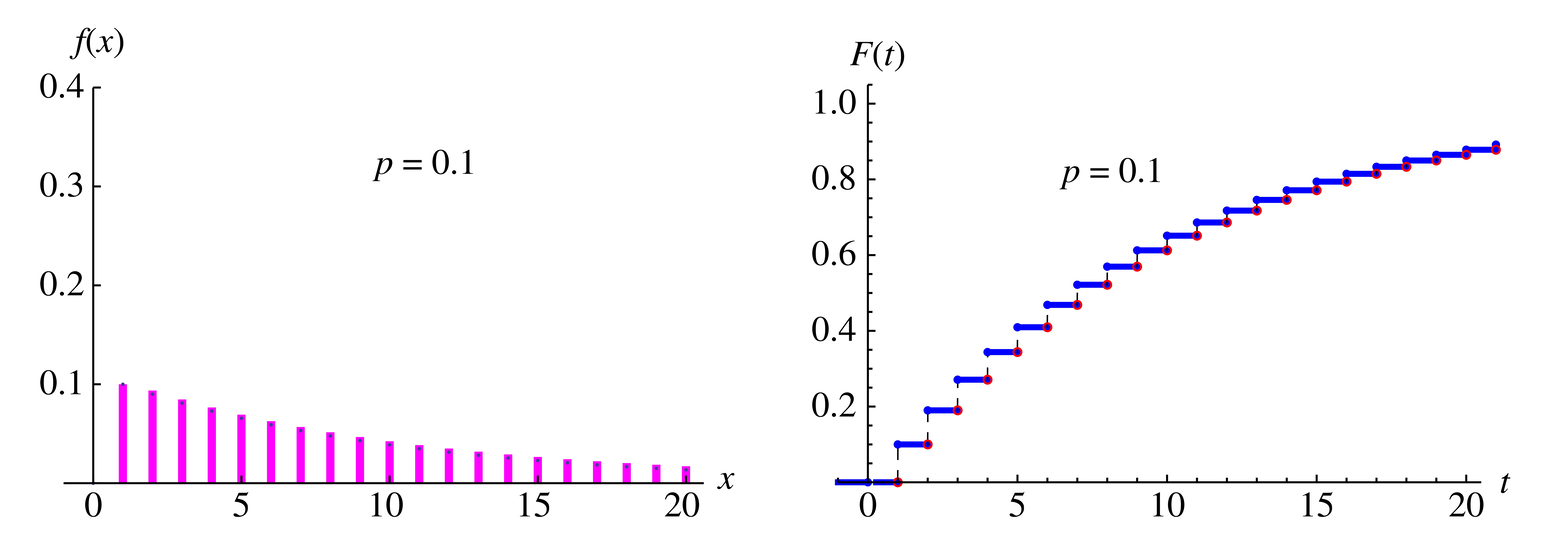
\includegraphics[width=1\linewidth]{geom.png}\caption{Geométrica $G(p)$}
		Número $n$ de ensayos de Bernoulli independientes con la misma probabilidad de éxito $p$, hasta obtener el primer éxito.
		\begin{equation}
		\begin{matrix}
		f(x)=q^{x-1},\\
		x=1,2,\ldots,n;\\
		E(X)=\frac{1}{p},\ Var(X)=\frac{q}{p^2}
		\end{matrix}
		\end{equation}
	\end{subfigure}
	\begin{subfigure}[t]{.5\textwidth}
		\includegraphics[width=.95\linewidth]{negativabinominal.png}\caption{Negativa binominal $Nb(rp)$}
		Número $n$ de ensayos de Bernoulli independientes con la misma probabilidad de éxito $p$, hasta obtener resultado número $r$.
		\begin{equation}
		\begin{matrix}
		f(x)=\binom{x-1}{r-1}p^rq^{x-r},\\
		r=r,r+1,r+2,\ldots,n;\\
		E(X)=\frac{r}{p},\ Var(X)=\frac{rq}{p^2}
		\end{matrix}
		\end{equation}
	\end{subfigure}\ \ \ \ 
\begin{subfigure}[t]{.5\textwidth}
		\includegraphics[width=.95\linewidth]{hyperg.png}\caption{Hipergeométrica $h(n;a,b)$}
		Muestra aleatoria tamaño $n$ de ``bolas blancas'' no reemplazada de un contenedor con $a$ blancas y $b$ negras.
		\begin{equation}
		\begin{matrix}
		f(x)=P(X=x)=\frac{num}{den}\\
		y\\
		z
		\end{matrix}
		\end{equation}
	\end{subfigure}	
	\begin{subfigure}[t]{.5\textwidth}
		\includegraphics[width=.95\linewidth]{gama.png}
		\caption{$\Gamma$}
	\end{subfigure}\ \ \ \ 
\begin{subfigure}[t]{.5\textwidth}\centering
		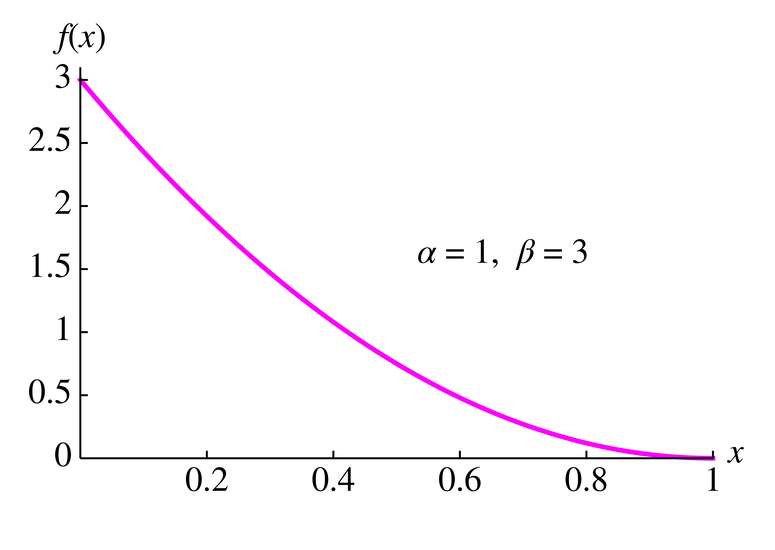
\includegraphics[width=.95\linewidth]{beta.png}\caption{Beta}
		blablabla
		\begin{equation}
		\begin{matrix}
		x\\
		y\\
		z
		\end{matrix}
		\end{equation}
	\end{subfigure}	
	\begin{subfigure}[t]{.5\textwidth}
		\includegraphics[width=.95\linewidth]{epsilon_lambda.png}
		\caption{$\epsilon(\lambda)$}
	\end{subfigure}\ \ \ \ 
\begin{subfigure}[t]{.5\textwidth}
		\includegraphics[width=.95\linewidth]{normal.png}\caption{Normal}
		blablabla
		\begin{equation}
		\begin{matrix}
		x\\
		y\\
		z
		\end{matrix}
		\end{equation}
	\end{subfigure}	
	\begin{subfigure}[t]{.5\textwidth}
		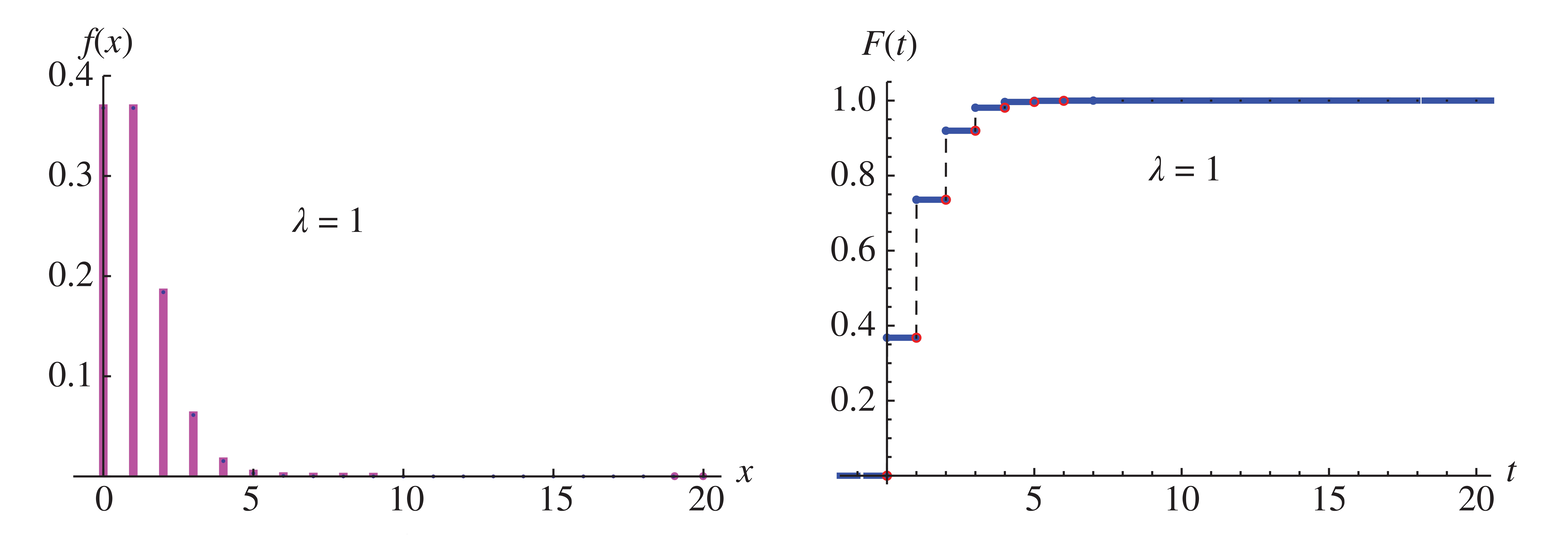
\includegraphics[width=.95\linewidth]{poisson.png}\caption{Poisson}
		blablabla
		\begin{equation}
		\begin{matrix}
		x\\
		y\\
		z
		\end{matrix}
		\end{equation}
	\end{subfigure}\ \ \ \ 
\begin{subfigure}[t]{.5\textwidth}
		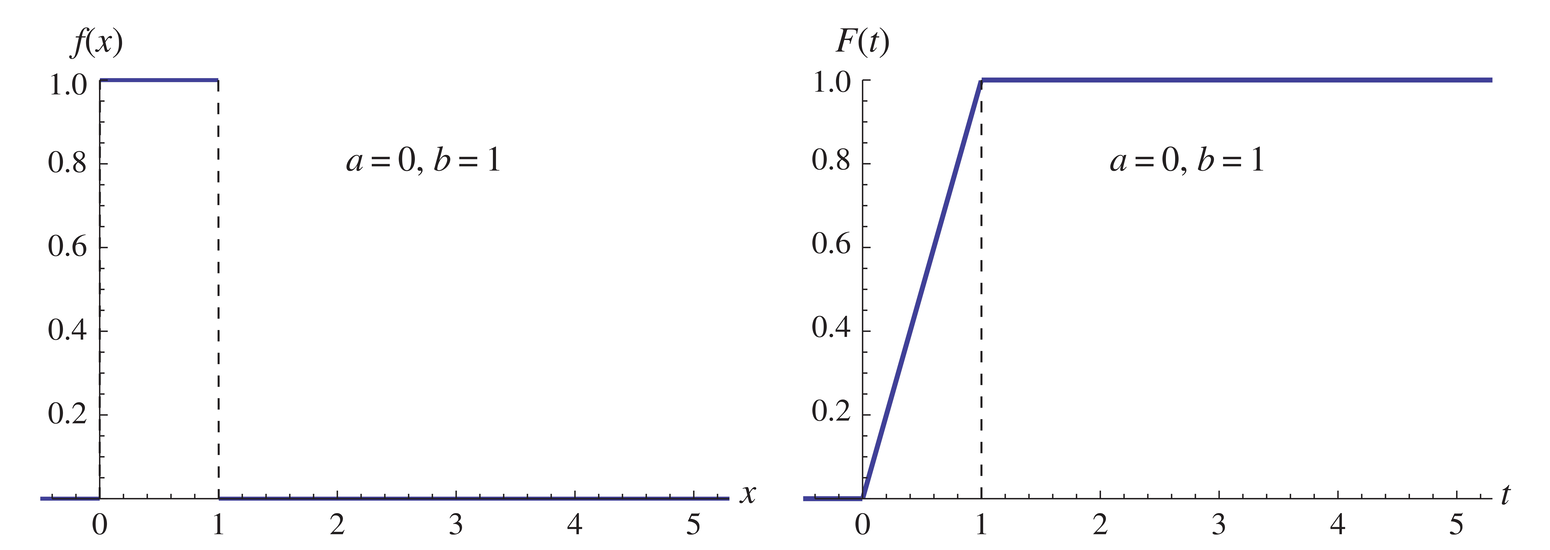
\includegraphics[width=.95\linewidth]{uniforme.png}\caption{Uniforme}
		blablabla
		\begin{equation}
		\begin{matrix}
		x\\
		y\\
		z
		\end{matrix}
		\end{equation}
	\end{subfigure}
\end{figure}
\#\#\#\#\#\#\#\#\#\#\#\#\#\#\#\#\#\#\#\#\#\#\#\#\#\#\#\#\#\#\#\#\#\#\#\#\#\#\#\#
\begin{center}sup\end{center}

\#\#\#\#\#\#\#\#\#\#\#\#\#\#\#\#\#\#\#\#\#\#\#\#\#\#\#\#\#\#\#\#\#\#\#\#\#\#\#\#\\
\subsubsection {Distribución de Bernoulli y binominal}
Una variable aleatoria tiene la \emph{distribución de Bernoulli} con un parámetro $p$ si $P(X=1)=p$ y $P(X=0=1-p)$, cuando $0<p<1$. Se escribe como $X \sim Bern(p)$, el símbolo $\sim$ significa ``distribuido como'' y la probabilidad $p$ es el \emph{parámetro}, que determina qué distribución de Bernoulli específica tenemos.

Supóngase que se realizan $n$ ensayos Bernoulli independientes, cada uno con probabilidad $p$ de éxito. $X$ sea el número de éxitos, la distribución $X$ se llama \emph{distribución binominal} con parámetros $n$ y $p$; se escribe $X \sim Bin(p,n)$.
$Bern(p)$ es la misma distribución que $Bin(1,p)$. Bernoulli es un caso especial de binominal, si $x \sim Bin(1,p)$, entonces la función de probabilidad de $X$ es
\begin{equation}
P(X=k)=\binom{n}{k}p^k(1-p)^{n-k}
\end{equation}
para $k=0,1,\ldots,n$ (y por otra parte $P(X=k)=0$).
\subsubsection {Distribución de hipergeométrica}
Si $X \sim HGeom(w,b,n)$, entonces la función de probabilidad de X es
\begin{equation}
P(X=k)=\frac{\binom{w}{k}\binom{b}{n-k}}{\binom{w+b}{n}},
\end{equation}
para enteros $k$ satisfaciendo $0\leq k\leq w$ y $0\leq n-k\leq b$, y $P(X=k)=0$. La estructura esencial de la distribución hipergeométrica se basa en que objetos en su población están clasificados usando dos tipos de etiquetas, al menos una de estas siendo asignada al azar.
Las distribuciones $HGeom(w,b,n)$ y $HGeom(n,w+b-n,1)$ son idénticas si $X$ y $Y$ tienen la misma distribución, podemos demostrarlo algebraicamente:
\begin{equation}
P(X=k)=\frac{\binom{w}{k}\binom{b}{n-k}}{\binom{w+b}{n}}=\frac{w!b!n!(w+b-n)!}{k!(w+b)!(w-k)!(n-k)!(b-n+k)!}
\end{equation}
\begin{equation}
P(X=k)=\frac{\binom{n}{k}\binom{w+b-n}{w-k}}{\binom{w+b}{w}}=\frac{w!b!n!(w+b-n)!}{k!(w+b)!(w-k)!(n-k)!(b-n+k)!}.
\end{equation}%if intro for bernolli and hyper neede, 3.4.6 has a bit a few useful lines
\subsubsection {Distribución uniforme discreta}
Teniendo $C$, un conjunto finito no vacío de números, se elige un número uniformemente al azar (o sea que todos los números tienen la misma posibilidad de ser elegidos), llámese $X$. Entonces se dice que $X$ una \emph{distribución uniforme discreta} con el parámetro $C$. Se dice entonces que la función de probabilidad de $X \sim DUNif(C)$ (la distribución uniforme discreta de $X$) es
\begin{equation}
P(X=x)=\frac{1}{|C|}
\end{equation}
para $x \in C$ (de lo contrario $0$) ya que la función de probabilidad debe sumar 1.
\subsection {distribuciones}\label{subsec:dd}%\subsubsection{LOTUS}
%La \emph{ley del estadista inconsciente} (\emph{LOTUS}, por sus siglas en inglés) permite calcular $E(g(X))$ directamente usando la distribución de $X$, sin tener que encontrar la distribución de $g(X)$ primero: si $X$ es una variable discreta y $g$ es una función de $\mathbb{R}$ a $\mathbb{R}$, entonces
%\begin{equation}
%E(g(X))=\sum_{x}g(x)P(X=x),
%\end{equation}
%donde la suma se toma de todos los valores posibles de $X$. El valor esperado de $g(X)$ puede ser escrito en forma no agrupado como
%\begin{equation}
%E(g(X))=\sum_{s}g(X(s))p(\{s\}).
%\end{equation}
%\subsubsection{Varianza, agregarlas a la secc que pertenecen}
%Varianza de la geométrica (agregarla a la geom después de editar todo y hacerlo más breve)
%\begin{equation}
%Var(X)=E(X^2)-{(EX)}^2=\frac{q(1+q)}{p^2}-{(\frac{q}{p})}^2=\frac{q}{p^2}
%\end{equation}
%Varianza de la geométrica (lo mismo)
%\begin{equation}
%Var(X)=E(X^2)-{(EX)}^2=(n(n-1)p^2+np)-(np)^2=np(1-p).
%\end{equation}
%Una variable aleatoria $X$ tiene \emph{distribución de Poisson} (denotada $X\sim Pois(\lambda)$) con el parámetro $\lambda$, cuando $\lambda > 0$ si la PMF de $x$ es
%\begin{equation}
%P(X=k)=\frac{e^{-\lambda}\lambda^k}{k!}, k=0,1,2,\ldots.
%\end{equation}
%Varianza de la distribución de Poisson es
%\begin{equation}
%Var(X)=E(X^2)-{(EX)}^2=\lambda(1+\lambda)-\lambda^2=\lambda
%\end{equation}

\emph{Inteligencia artificial} es definida como ``el esfuerzo por automatizar tareas intelectuales normalmente realizadas por humanos''\cite{cho18}, de este campo general se desprenden el \emph{aprendizaje maquinal} y el \emph{aprendizaje profundo}.
%\section {Objetivos}\label{sec:objetivos}\section {Objetivos}
\subsection {General}
Haciendo uso de las ciencias de la computación, las herramientas matemáticas de estadística y métodos de aprendizaje autónomo, se busca obtener información cuantitativa de textos. La fuente de información será redes sociales, cadenas noticiosas y audio de programas de capacitación, para inferir posiciones, tendencias, comportamientos o razones de grupos sociales. El de trabajo es clasificación, estimación, detección y comprobación.
\subsection {Particulares}
\begin{enumerate}
    \item Desarrollar un modelo de base de datos que permita la captura de categorías para un determinado problema, los elementos de identificación de cada categoría, el origen de la información y su correlación.
    \item Construir una estructura de datos que capte la estimación o valores esperados para el procesamiento de textos.
    \item Elaborar un sistema de objetos para el soporte de los elementos de aprendizaje autónomo.
    \item Generar los elementos de captura de textos para su almacenamiento y procesamiento.
    \item Elaborar un modelo estadístico que permita comprobar las estimaciones a partir de los datos y en consecuencia realizar un ajuste en los parámetros usados para el aprendizaje autónomo.
    \item Producir los reportes con un análisis estadístico que faciliten la interpretación de resultados y den pauta para la obtención del conocimiento de interés.
\end{enumerate}
\section {Metas científicas}
La meta de este proyecto es -la integración -de elementos de estad, ciencia comp, apr autónomo(ML) para procesamiento de lenguage natural (PLN).
%\section {Metodologías}\label{sec:metod}
%\section {Referencias}\label{sec:refs}
%\printbibliography[heading=none]
\end{document}

%AAAAAAAAAAAAAAAAAAAAAAAAAAAAAAAAAAAAAAAAAAAAAAAA\\
%AAAAAAAAAAAAAAAAAAAAAAAAAAAAAAAAAAAAAAAAAAAAAAAAAA\\
%AAAAAAAAAAAAAAAAAAAAAAAAAAAAAAAAAAAAAAAAAAAAAAAAAA\\